\newpage
\section{Teilversuch 4: Messung der Resonanzkurve für eine Oberschwingung}
	\subsection{Messreihe}
	Fehler der Frequenzen $\Delta f = \SI{1}{\hertz}$ \\
	Fehler der Spannung $\Delta f = \SI{0.2}{\milli\volt}$

	Raumhintergrund $= \SI{1.1(2)}{\milli\volt}$

	\begin{center}
		\begin{tabular}{l *{10}{r}}
			\toprule
			$f / \si{\hertz}$ & \num{1011} & \num{980} & \num{970} & \num{952} & \num{928} & \num{910} & \num{892} & \num{881} & \num{871} & \num{861} \\
			\midrule
			$U_\text{eff} / \si{\milli\volt}$ & \num{7.33} & \num{7.53} & \num{7.99} & \num{8.85} & \num{10.85} & \num{13.45} & \num{18.33} & \num{23.31} & \num{30.14} & \num{44.53} \\
			\bottomrule
			\toprule
			$f / \si{\hertz}$ & \num{854} & \num{850} & \num{844} & \num{841} & \num{837} & \num{833} & \num{830} & \num{825} & \num{818} & \num{810} \\
			\midrule
			$U_\text{eff} / \si{\milli\volt}$ & \num{64.33} & \num{85.80} & \num{125.53} & \num{149.11} & \num{149.49} & \num{120.65} & \num{96.04} & \num{71.73} & \num{54.43} & \num{41.24} \\
			\bottomrule
			\toprule
			$f / \si{\hertz}$ & \num{801} & \num{790} & \num{780} & \num{760} & \num{742}  \\
			\midrule
			$U_\text{eff} / \si{\milli\volt}$ & \num{34.00} & \num{28.51} & \num{25.66} & \num{22.68} & \num{21.61} \\
			\bottomrule
		\end{tabular}
	\end{center}

	\subsection{Graph}
	Aus der Anleitung des Versuchs MOS lässt die folgende Funktion eine Resonanzkurve beschreiben:
	\begin{equation}
		\hat{x} = \frac{\omega_0^2}{\sqrt{\pbrace{\omega_0^2 - \omega^2}^2+\pbrace{2\beta\omega}^2}}~\hat{x}_\text{A} \iff U_\text{eff} = \frac{f_0^2}{\sqrt{\pbrace{f_0^2 - f^2}^2+\pbrace{2\beta f}^2}}~U_\text{A}
	\end{equation}

	Da die Kurvenanpassung mit \gnuplot{} sehr empfindlich auf die Wahl der Startparameter reagiert, müssen die Startparameter sorgfältig ausgewählt. Dafür ist eine grobe Kurveanpassung wie im Versuch MOS mittels Geogebra per Hand durchgeführt:
	\begin{figure}[H]
		\centering
		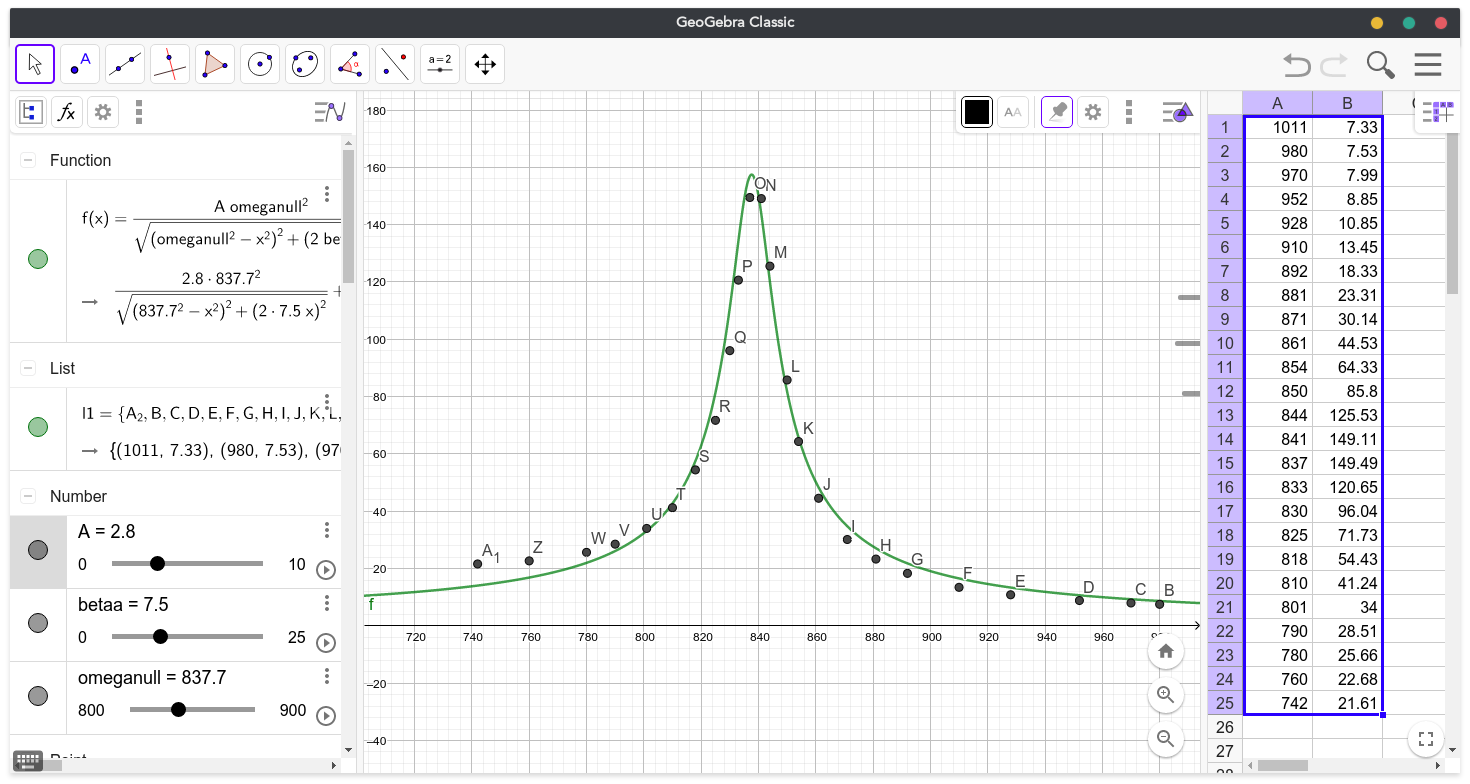
\includegraphics[width=0.9\textwidth]{geogebra.png}
		\caption{Grobe Kurveanpassung mittels Geogebra}
	\end{figure}

	Der Raumhintergrund und dessen Fehler sind direkt im \gnuplot{} Skript berücksichtigt (Siehe Appendix \ref{appdx:gnuplotTV4}). Der Fehler der Spannung nach dem Abzug des Raumhintergrund wird als $(\SI{0.2}{\milli\volt} + \SI{0.2}{\milli\volt} = \SI{0.4}{\milli\volt})$ angenommen. Der Grund dafür ist, dass wir letztendlich nur eine Messung von der Raumhintergrund haben, obwohl wir bei mehrfache Messungen eher Schwankungen gegen die gleiche Werten bekommen. Daher ist es sicherer bei der Kurvenanpassung einen größeren Fehler zu benutzen.

	\begin{figure}[H]
		\centering
		% GNUPLOT: LaTeX picture with Postscript
\begingroup
  \makeatletter
  \providecommand\color[2][]{%
    \GenericError{(gnuplot) \space\space\space\@spaces}{%
      Package color not loaded in conjunction with
      terminal option `colourtext'%
    }{See the gnuplot documentation for explanation.%
    }{Either use 'blacktext' in gnuplot or load the package
      color.sty in LaTeX.}%
    \renewcommand\color[2][]{}%
  }%
  \providecommand\includegraphics[2][]{%
    \GenericError{(gnuplot) \space\space\space\@spaces}{%
      Package graphicx or graphics not loaded%
    }{See the gnuplot documentation for explanation.%
    }{The gnuplot epslatex terminal needs graphicx.sty or graphics.sty.}%
    \renewcommand\includegraphics[2][]{}%
  }%
  \providecommand\rotatebox[2]{#2}%
  \@ifundefined{ifGPcolor}{%
    \newif\ifGPcolor
    \GPcolortrue
  }{}%
  \@ifundefined{ifGPblacktext}{%
    \newif\ifGPblacktext
    \GPblacktexttrue
  }{}%
  % define a \g@addto@macro without @ in the name:
  \let\gplgaddtomacro\g@addto@macro
  % define empty templates for all commands taking text:
  \gdef\gplbacktext{}%
  \gdef\gplfronttext{}%
  \makeatother
  \ifGPblacktext
    % no textcolor at all
    \def\colorrgb#1{}%
    \def\colorgray#1{}%
  \else
    % gray or color?
    \ifGPcolor
      \def\colorrgb#1{\color[rgb]{#1}}%
      \def\colorgray#1{\color[gray]{#1}}%
      \expandafter\def\csname LTw\endcsname{\color{white}}%
      \expandafter\def\csname LTb\endcsname{\color{black}}%
      \expandafter\def\csname LTa\endcsname{\color{black}}%
      \expandafter\def\csname LT0\endcsname{\color[rgb]{1,0,0}}%
      \expandafter\def\csname LT1\endcsname{\color[rgb]{0,1,0}}%
      \expandafter\def\csname LT2\endcsname{\color[rgb]{0,0,1}}%
      \expandafter\def\csname LT3\endcsname{\color[rgb]{1,0,1}}%
      \expandafter\def\csname LT4\endcsname{\color[rgb]{0,1,1}}%
      \expandafter\def\csname LT5\endcsname{\color[rgb]{1,1,0}}%
      \expandafter\def\csname LT6\endcsname{\color[rgb]{0,0,0}}%
      \expandafter\def\csname LT7\endcsname{\color[rgb]{1,0.3,0}}%
      \expandafter\def\csname LT8\endcsname{\color[rgb]{0.5,0.5,0.5}}%
    \else
      % gray
      \def\colorrgb#1{\color{black}}%
      \def\colorgray#1{\color[gray]{#1}}%
      \expandafter\def\csname LTw\endcsname{\color{white}}%
      \expandafter\def\csname LTb\endcsname{\color{black}}%
      \expandafter\def\csname LTa\endcsname{\color{black}}%
      \expandafter\def\csname LT0\endcsname{\color{black}}%
      \expandafter\def\csname LT1\endcsname{\color{black}}%
      \expandafter\def\csname LT2\endcsname{\color{black}}%
      \expandafter\def\csname LT3\endcsname{\color{black}}%
      \expandafter\def\csname LT4\endcsname{\color{black}}%
      \expandafter\def\csname LT5\endcsname{\color{black}}%
      \expandafter\def\csname LT6\endcsname{\color{black}}%
      \expandafter\def\csname LT7\endcsname{\color{black}}%
      \expandafter\def\csname LT8\endcsname{\color{black}}%
    \fi
  \fi
    \setlength{\unitlength}{0.0500bp}%
    \ifx\gptboxheight\undefined%
      \newlength{\gptboxheight}%
      \newlength{\gptboxwidth}%
      \newsavebox{\gptboxtext}%
    \fi%
    \setlength{\fboxrule}{0.5pt}%
    \setlength{\fboxsep}{1pt}%
\begin{picture}(8640.00,5760.00)%
    \gplgaddtomacro\gplbacktext{%
      \csname LTb\endcsname%%
      \put(814,704){\makebox(0,0)[r]{\strut{}$0$}}%
      \put(814,1253){\makebox(0,0)[r]{\strut{}$20$}}%
      \put(814,1803){\makebox(0,0)[r]{\strut{}$40$}}%
      \put(814,2352){\makebox(0,0)[r]{\strut{}$60$}}%
      \put(814,2902){\makebox(0,0)[r]{\strut{}$80$}}%
      \put(814,3451){\makebox(0,0)[r]{\strut{}$100$}}%
      \put(814,4000){\makebox(0,0)[r]{\strut{}$120$}}%
      \put(814,4550){\makebox(0,0)[r]{\strut{}$140$}}%
      \put(814,5099){\makebox(0,0)[r]{\strut{}$160$}}%
      \put(946,484){\makebox(0,0){\strut{}$700$}}%
      \put(1988,484){\makebox(0,0){\strut{}$750$}}%
      \put(3031,484){\makebox(0,0){\strut{}$800$}}%
      \put(4073,484){\makebox(0,0){\strut{}$850$}}%
      \put(5116,484){\makebox(0,0){\strut{}$900$}}%
      \put(6158,484){\makebox(0,0){\strut{}$950$}}%
      \put(7201,484){\makebox(0,0){\strut{}$1000$}}%
      \put(8243,484){\makebox(0,0){\strut{}$1050$}}%
    }%
    \gplgaddtomacro\gplfronttext{%
      \csname LTb\endcsname%%
      \put(209,2901){\rotatebox{-270}{\makebox(0,0){\strut{}Mikrofonspannung $U_\text{eff}$ ($\si{\milli\volt}$)}}}%
      \put(4594,154){\makebox(0,0){\strut{}Frequenz $f$ ($\si{\hertz}$)}}%
      \put(4594,5429){\makebox(0,0){\strut{}Resonanzkurve des Rohres bei der 2. Oberschwingung}}%
      \csname LTb\endcsname%%
      \put(7256,4926){\makebox(0,0)[r]{\strut{}Angepasste Kurve}}%
      \csname LTb\endcsname%%
      \put(7256,4706){\makebox(0,0)[r]{\strut{}Messpunkte}}%
    }%
    \gplbacktext
    \put(0,0){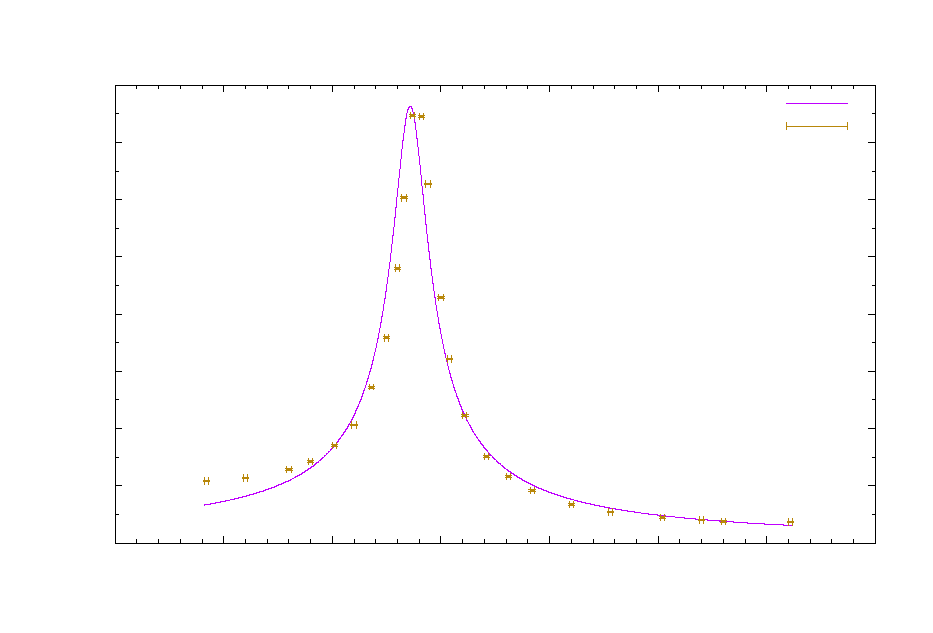
\includegraphics{tv4-plot}}%
    \gplfronttext
  \end{picture}%
\endgroup

		\caption{\centering Messung der Resonanzkurve des Rohres bei der 2. Oberschwingung\captionbr $\chi^2_{\text{red}} = \num{32.6373} > 1 \implies$ Schlechte Anpassung}
		\label{fig:tvfour-plot}
		\vspace{-1em}
	\end{figure}
	Als Endergebnis erhalten wir:
	\begin{center}
		\begin{tabular}{l r r}
			\toprule
			Variable & Rohausgabe & Gerundet \\
			\midrule
			$f_0$ & \SI{835.89(146)}{\hertz} & \SI{835.9(15)}{\hertz} \\
			$U_\text{A}$ & \SI{2.8473(1317)}{\milli\volt} & \SI{2.85(14)}{\milli\volt} \\
			$\beta$ & \num{7.79(102)} & \num{7.8(11)} \\
			\bottomrule
		\end{tabular}
	\end{center}

	Anstatt einfach die Messpunkte durch eine glatte Kurve zu verbinden, war eine theoretische Kurve auf die Messwerte angepasst. Die Anpassung war leider schlecht, und der Grund dafür liegt vermütlich daran, dass wir Nebeneffekte bzw. andere Faktoren nicht berücksichtigt haben. Es könnte auch sein, dass wir alle Werten im SI Einheiten skalieren sollten, bevor wir die Kurvenanpassung durchführen. 

	Unsere gemessene Resonanzfrequenz $f_0 = \SI{837(1)}{\hertz}$ liegt auch im Fehlerintervall des aus der Kurvenanpassung gefundene $f_0$. Die Werte stimmen also miteinander überein.